\chapter{On finding app case study projects}
This appendix provides some guidance for finding app case studies for existing real world mobile apps. One of the aims of including this appendix is to help improve the repeatability of the work described in this thesis.

\section{case study procedure}
\subsection{Exploration and selection}
\begin{wrapfigure}{R}{0.5\textwidth}
  \begin{center}
    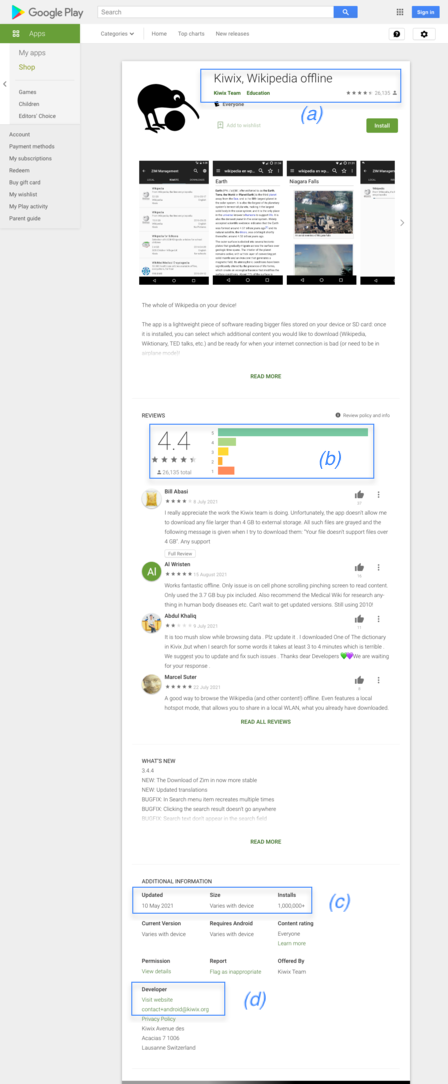
\includegraphics[width=0.42\textwidth]{images/google-play/annotated-resized40pct-2021-09-30-kiwix-app-on-google.png}
  \end{center}
  \caption{Kiwix: app presented in Google Play Store}
  \label{fig:gp-kiwix-app}
\end{wrapfigure}

Various forms of exploration are available. For apps in major app stores the app store may provide pertinent information that can be used to preliminarily select target apps. Figure~\ref{fig:gp-kiwix-app} is how the Kiwix Android app appears to visitors to Google Play when using a web browser (Firefox in this example). Four areas of pertinent information have been highlighted:

\begin{enumerate}[label=(\alph*)]
    \itemsep0em
    \item The category of the app and the count of ratings. The category helps group case studies by category, and also helps compare a particular app with the median crash and ANR rates for apps in that category. More details on these are available in \secref{section-peer-categories}.
    \item More details of the distribution of the ratings.
    \item When the app was last updated in the app store and the number of installs of all versions of this app.
    \item Contact details for the developer~\footnote{That said, like many relationships, a warm lead is more likely to elicit a response than a cold email to the published email address. For this research all bar one of the case studies was established through a warm lead, someone who knows me. The exception was the \href{https://github.com/Phantast/smartnavi}{Smartnavi} project where the connection was established through email.}.
\end{enumerate}

Recruiting candidates: \citepalt{Ko2015_a_practical_guide_to_controlled_experiments_of_sw_eng_tools_with_human_participants} provides sound general advice on recruiting candidates which may be useful.